\chapter{The Problem of Being Inside the System}
\label{chap:problem-of-being-inside}

\section{The Internal Perspective}

Physics has a fundamental problem: we are trying to describe a system from the inside.

At least, it certainly appears that way.
We seem to live in a vast geometric space in which we are small.
In the language of set theory, we are the small subset $O$ attempting to map the superset $U$.

\begin{figure}[h]
    \centering
    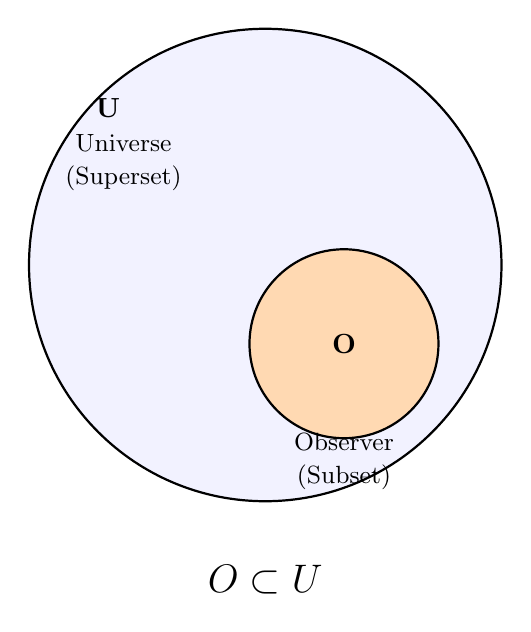
\begin{tikzpicture}
        % The Universe U
        \draw[thick, fill=blue!5] (0,0) circle (3cm);
        \node at (-2,2) {\textbf{U}};
        \node[text width=2.2cm, align=center] at (-1.8,1.3) {\small Universe\\(Superset)};

        % The Observer O
        \draw[thick, fill=orange!30] (1,-1) circle (1.2cm);
        \node at (1,-1) {\textbf{O}};
        \node[text width=2cm, align=center] at (1,-2.5) {\small Observer\\(Subset)};

        % The Notation
        \node at (0,-4) {\Large $O \subset U$};
    \end{tikzpicture}
    \caption{The problem of internal perspective: $O$ is a subset of $U$.}
\end{figure}

Because we are embedded within reality, we cannot help but perceive it through a human lens.
We experience ``time'' as a flow and ``matter'' as solid, yet it now appears increasingly likely that these are artifacts of our vantage point.
This makes it extraordinarily difficult to distinguish between a fundamental law of nature and a mere byproduct of perspective.
We are not external spectators watching a machine; we are observers whose own bodies are being ground between its gears.

The intuition that we are mere subsets of the universe feels correct.
We want to believe that the cosmos would exist exactly as it is even if we had never appeared.
It feels almost arrogant to suggest that our thin layer of gray matter could play any role in the fundamental existence of the stars.

Even if the universe exists independently of us, our description of it---the physics we write down---is entirely filtered through our internal perspective.
We are trapped inside.


\section{The Method: Escaping the Trap}

If our conclusions from the previous chapters hold, there is a remarkable way out of this trap.

If the four axioms presented in Chapter~\nameref{chap:humans-as-axiomatic-systems} hold---that DNA is made of ordinary matter, humans are implementations of axiomatic systems, physical processes are Turing-computable, and subjective experiences like pain have measurable physical consequences---then humans and the universe are not made of mysterious, uncomputable ``magic,'' but of abstract information.

This allows us to turn the internal-perspective problem on its head.

If we are abstract information, and the medium does not matter, then an axiomatic system can be instantiated on a sheet of paper, in a human brain, or on a silicon chip.

We do not truly know what time is---likely because we are submerged within it.
However, while the essence of time remains elusive, its logic is something we can simulate.

Whatever mystery we fail to grasp about the flow of time or the feeling of pain would have to be present within the machine running the code.
We may not fully understand the cosmos, but we fully understand computers.

By moving the mystery into a block of silicon, we transform a metaphysical puzzle into a debuggable program.
Instead of looking at the universe from the inside, we can look at it from the outside.

